\documentclass[german,11pt]{beamer}
% ------------------------------------------------------------------------------
% Packages
\usepackage[german,english,french]{babel}
\usepackage[T1]{fontenc}
\usepackage[utf8]{inputenc}
\usepackage{ragged2e}
\usepackage[normalem]{ulem}


\usepackage{listings}
\usepackage{color}
\usepackage{xcolor} 
\usepackage{plantuml}
% \usepackage{enumitem} \setitemize{leftmargin=*}   // Keine Aufzählung
\usepackage{pgfplots}

\usepackage{csquotes}

\pgfplotsset{compat=1.18}

\definecolor{dkgreen} {rgb}{0,0.6,0}
\definecolor{gray}{rgb}{0.5,0.5,0.5}
\definecolor{mauve}{rgb}{0.58,0,0.82}

\lstset{frame=tb,
  language=Java,
  aboveskip=3mm,
  belowskip=3mm,
  showstringspaces=false,
  columns=flexible,
  basicstyle={\small\ttfamily},
  numbers=none,
  numberstyle=\tiny\color{gray},
  keywordstyle=\color{blue},
  commentstyle=\color{dkgreen},
  stringstyle=\color{mauve},
  breaklines=true,
  breakatwhitespace=true,
  tabsize=3
}
% ------------------------------------------------------------------------------
% Parameters
\mode<presentation>{\usetheme{Luebeck}}
\setbeamertemplate{itemize items}[triangle]
\setbeamercovered{transparent}
\usecolortheme{dove}
\usefonttheme{serif}
\addtobeamertemplate{block begin}{}{\justifying}
% ToC
\AtBeginSection[] {
  \begin{frame}{Inhalt}
    \tableofcontents[currentsection]
  \end{frame}
}
% Headline
\makeatletter
\setbeamertemplate{headline}{%
  \leavevmode%
  \@tempdimb=2.4375ex%
  \ifnum\beamer@subsectionmax<\beamer@sectionmax%
    \multiply\@tempdimb by\beamer@sectionmax%
  \else%
    \multiply\@tempdimb by\beamer@subsectionmax%
  \fi%
  \ifdim\@tempdimb>0pt%
    \advance\@tempdimb by 1.825ex%
    \begin{beamercolorbox}[wd=.5\paperwidth,ht=\@tempdimb]{section in head/foot}%
      \vbox to\@tempdimb{\hfill\insertsectionnavigation{.3\paperwidth}\vfil}%
    \end{beamercolorbox}%
    \begin{beamercolorbox}[wd=.3\paperwidth,ht=\@tempdimb]{subsection in head/foot}%
      \vbox to\@tempdimb{\vfil\insertsubsectionnavigation{.5\paperwidth}\vfil}%
    \end{beamercolorbox}%
    \begin{beamercolorbox}[wd=.2\paperwidth,ht=\@tempdimb]{subsection in head/foot}%
      \vbox to\@tempdimb{\vfil\hfill
\includegraphics[height=1cm]{fig/graphics/logo.jpg}\vfil}
    \end{beamercolorbox}%    
  \fi%
}
\makeatother
% Footline
\makeatletter
\setbeamertemplate{footline}{%
  \leavevmode%
  \hbox{\begin{beamercolorbox}[wd=.5\paperwidth,ht=2.5ex,dp=1.125ex,leftskip=.3cm,rightskip=.3cm]{author in head/foot}%
    \usebeamerfont{author in head/foot}\insertshortdate \hfill \insertshortauthor
  \end{beamercolorbox}%
  \begin{beamercolorbox}[wd=.5\paperwidth,ht=2.5ex,dp=1.125ex,leftskip=.3cm,rightskip=.3cm plus1fil]{title in head/foot}%
    \usebeamerfont{title in head/foot}\insertshorttitle \hfill \insertframenumber\,/\,\inserttotalframenumber
  \end{beamercolorbox}}%
  \vskip0pt%
}
\makeatother

\addto\captionsenglish{% Replace "english" with the language you use
  \renewcommand{\contentsname}%
    {Whatever}%
}

% ------------------------------------------------------------------------------
% Infos
\title[VS]{Verteilte Systeme}
%\subtitle[Short subtitle]{Subtitle}
\author[BCK]{Prof. Dr. Martin Becke}
\date[0.9]{Version 0.9}
\institute[CaDS]{CaDS - HAW Hamburg}
%\logo{
\includegraphics[height=1cm]{fig/graphics/logo.jpg}}
% ------------------------------------------------------------------------------

% Document
\begin{document}

% ------------------------------------------------------------------------------
% Titlepage
\begin{frame}
  \titlepage{}
\end{frame}
% ------------------------------------------------------------------------------
% ToC
%\begin{frame}{Contents}
%  \tableofcontents
%\end{frame}
% ------------------------------------------------------------------------------
\section{RPC} 
%\section{Einleitung}
\subsection{Remote Procedure Call}
\begin{frame}
  \frametitle{Remote Procedure Call}
  \framesubtitle{Idee}
  \begin{itemize}
    \item Ein Kommunikationsmodell
    \item Prozeduraufrufe zwischen Prozessen auf unterschiedlichen Systemen oder Maschinen
    \item Entfernte Funktionen oder Methoden aufrufen wie lokale
  \end{itemize}
\end{frame}


\begin{frame}
  \frametitle{Remote Procedure Call}
  \framesubtitle{Ablauf}
  \begin{enumerate} 
  \item Der Client ruft die entfernte Prozedur über den Client Stub auf, als wäre es eine lokale Funktion.
  \item Der Client Stub wandelt die Parameter der Anfrage in ein standardisiertes Format um (Marshalling) und sendet die Anfrage über das Kommunikationsprotokoll an den Server.
  \item Der Server Stub empfängt die Anfrage, demarshalled die Parameter und ruft die entsprechende Funktion auf dem Server auf.
  \item Die Funktion wird auf dem Server ausgeführt, und das Ergebnis wird an den Server Stub zurückgegeben.
  \item Der Server Stub marshallt das Ergebnis und sendet es über das Kommunikationsprotokoll an den Client Stub zurück.
  \item Der Client Stub empfängt die Antwort, demarshalled das Ergebnis und gibt es an den Client zurück.
  \end{enumerate}
\end{frame}

\begin{frame}
  \frametitle{Remote Procedure Call}
  \framesubtitle{Naiver Entwurf}
  \begin{figure}[!ht]
    \centering
    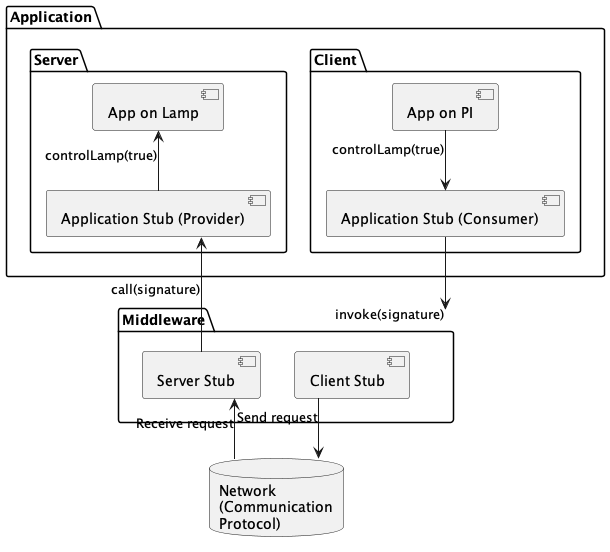
\includegraphics[width=0.55\textwidth]{fig/uml/rpc-simple.png}
    \caption{Erster Ansatz einer RPC Architektur}
    \label{fig:simple-rpc}
  \end{figure}
\end{frame}

\begin{frame}[fragile]
  \frametitle{Remote Procedure Call}
  \framesubtitle{Naiver Code I}
  \begin{minipage}{\textwidth}
  \begin{lstlisting}[caption={RPC Interface},captionpos=b,label={lst:rpc-interface}]
  public interface Lamp {
      void controlLamp(Boolean b);
  }
  \end{lstlisting}
  \end{minipage}
\end{frame}

\begin{frame}[fragile]
  \frametitle{Remote Procedure Call}
  \framesubtitle{Naiver Code II}
  \begin{minipage}{\textwidth}
  \begin{lstlisting}[caption={RPC Remote Implementation},captionpos=b,label={lst:rpc-remote}]
  public class LampRemote implements Lamp {
      @Override
      public void controlLamp(boolean b){
        List<Boolean> list = new ArrayList<Boolean>(); 
          Collections.addAll(list, b);
          Middleware.invoke("controlLamp", list);
      }
  }
  \end{lstlisting}
  \end{minipage}
\end{frame}

\begin{frame}[fragile]
  \frametitle{Remote Procedure Call}
  \framesubtitle{Naiver Code III}
  \begin{minipage}{\textwidth}
  \begin{lstlisting}[caption={Application Stub mit Factory Pattern},captionpos=b,label={lst:rpc-factory}]
  public class LampFactory {
      public static Lamp createLamp() {
          // Hier koennte die Middleware-Verbindung hergestellt werden.
          // In diesem Beispiel verwenden wir eine einfache lokale Implementierung.
          return new LampRemote();
      }
  }
  \end{lstlisting}
  \end{minipage}
\end{frame}

\begin{frame}[fragile]
  \frametitle{Remote Procedure Call}
  \framesubtitle{Naiver Code IV}
  \begin{minipage}{\textwidth}
  \begin{lstlisting}[caption={Controller ruft Middleware},captionpos=b,label={lst:rpc-controller}]
  public class LampController {
    public static void main(String[] args) {
          // Erstelle eine Lampe ueber die Factory-Methode (Application-Stub)
          Lamp lamp = LampFactory.createLamp();

          // Verwende die Lampe in der Anwendung
          lamp.controlLamp(true);
      }
  }
  \end{lstlisting}
  \end{minipage}
\end{frame}

\begin{frame}
  \frametitle{Remote Procedure Call}
  \framesubtitle{Marshalling Process - Beispiel}
  \begin{itemize} 
  \item Konvertierung Parameter (z.B. String und Integer) in ein plattformunabhängiges Format, z. B. Byte-Arrays.
  \item Hinzufügen von Metadaten, wie Typinformationen, zur Identifizierung der Parameter auf der Empfängerseite.
  \item Zusammenpacken der Byte-Arrays und Metadaten in einer Nachricht, die über das Netzwerk gesendet werden kann
  \end{itemize} 
\end{frame}

\begin{frame}
  \frametitle{Remote Procedure Call}
  \framesubtitle{Copy in, Copy out}
  \begin{itemize} 
  \item Semantik zur Übergabe von Parametern 
  \item Kopiert Parameter in eine Nachricht (Ohne Kenntnis der Daten)
  \item Benötigt ein generisches Regelwerk für Datentypen
  \item Alternative: Call by Reference - Direkter Speicherzugriff fremder Systeme
  \end{itemize} 
\end{frame}

\begin{frame}
  \frametitle{Remote Procedure Call}
  \framesubtitle{Copy in, Copy out Optimierung}
  \begin{itemize} 
  \item Datenkompression
  \item Effiziente Serialisierungsformate (Beispiel MessagePack)
  \item Selektive Übertragung
  \end{itemize} 
\end{frame}

\begin{frame}
  \frametitle{Remote Procedure Call}
  \framesubtitle{ Interface Definition Language (IDL)}
  \begin{itemize} 
  \item IDL beschreibt die Signatur der entfernten Funktionen
  \item Generierung des Stub- und Skeleton-Code aus der IDL-Definition
  \item Kann mit Code-Generator verbunden werden.
  \end{itemize} 
\end{frame}

\begin{frame}[fragile]
  \frametitle{Remote Procedure Call}
  \framesubtitle{IDL Example}
  \begin{minipage}{\textwidth}
  \begin{lstlisting}[caption={IDL Example},captionpos=b,label={lst:idl-example}]
  interface MathService {
    int add(in int a, in int b);
  }
  \end{lstlisting}
  \end{minipage}
\end{frame}

\begin{frame}[fragile]
  \frametitle{Remote Procedure Call}
  \framesubtitle{RPC IDL Service Impl}
  \begin{minipage}{\textwidth}
  \begin{lstlisting}[caption={RPC IDL Service Impl},captionpos=b,label={lst:idl-impl}]
  class MathServiceImpl(MathService):
      def add(self, a, b):
          return a + b
  \end{lstlisting}
  \end{minipage}
\end{frame}

\begin{frame}[fragile]
  \frametitle{Remote Procedure Call}
  \framesubtitle{RPC IDL Service Impl}
  \begin{minipage}{\textwidth}
  \begin{lstlisting}[caption={RPC IDL Service Impl},captionpos=b,label={lst:idl-impl-service}]
  math math_service_client = MathServiceStub(server_address)
  result = math_service_client.add(5, 7)
  print("Result of 5 + 7:", result)
  \end{lstlisting}
  \end{minipage}
\end{frame}

\begin{frame}
  \frametitle{Remote Procedure Call}
  \framesubtitle{Framework Beispiele}
  \begin{itemize} 
  \item XML-RPC \url{http://xmlrpc.com/}
  \item JSON-RPC \url{https://www.jsonrpc.org/}
  \item gRPC \url{https://grpc.io/}
  \end{itemize} 
\end{frame}

\begin{frame}[fragile]
  \frametitle{Remote Procedure Call}
  \framesubtitle{Beispiele XML-RPC}
  \begin{minipage}{\textwidth}
  \begin{lstlisting}[caption={XML-RPC in Python},captionpos=b,label={lst:xmp-rpc-python}]
  from xmlrpc.server import SimpleXMLRPCServer

  def add(a, b):
      return a + b

  server = SimpleXMLRPCServer(("localhost", 8080))
  server.register_function(add, "add")
  server.serve_forever()
  \end{lstlisting}
  \end{minipage}
\end{frame}

\begin{frame}
  \frametitle{Remote Procedure Call}
  \framesubtitle{Server-Stub, Skeleton und Server-Proxy}
  \begin{itemize} 
  \item Skeleton ist die reine Funktion
  \item Server-Stub ist das Skeleton aus der IDL abgleitet
  \item Server-Proxy übernimmt weitere Aufgaben wie diskutiert
  \end{itemize} 
\end{frame}
\subsection{Remote Method Invocation}
\begin{frame}
  \frametitle{Remote Method Invocation (RMI) }
  \framesubtitle{Idee}
  \begin{itemize} 
  \item Speziell für eine Objekt-orientierte Programmiersprache 
  \item Properitäte Protokolle
  \item In Java ist RMI eingebettet (Beispiel Script)
  \end{itemize} 
\end{frame}
\section{Chord}

%\subsection{Architek}
\begin{frame}
  \frametitle{P2P Chord}
  \framesubtitle{Idee}
  \begin{itemize}
    \item Chord-Architektur ist ein verteiltes Hashtabelle-System
    \item Basiert auf strukturierten Overlay-Netzwerk
    \item Bekannt seit 2001
    \item Grundlage für die Entwicklung von Blockchain-Technologien 
    \item Grundlage dezentralisierten autonomen Organisationen (DAOs) 
  \end{itemize}
\end{frame}

\begin{frame}
  \frametitle{P2P Chord}
  \framesubtitle{Struktur und Funktionsweise}
  \begin{itemize}
    \item Identifier Space: Default Ring
    \item Key-Node Mapping
    \item Finger Tables
    \item Lookup-Operationen
    \item Dynamik und Fehlertoleranz
  \end{itemize}
\end{frame}

\begin{frame}
  \frametitle{P2P Chord}
  \framesubtitle{Einsatzmöglichkeiten}
  \begin{itemize}
    \item Dateifreigabe
    \item Distributed Domain Name System (DDNS)
    \item Content Distribution Networks (CDN)
    \item Distributed Databases
    \item etc
  \end{itemize}
\end{frame}

\begin{frame}
  \frametitle{P2P Chord}
  \framesubtitle{Beispiel}
  \begin{figure}[!ht]
    \centering
    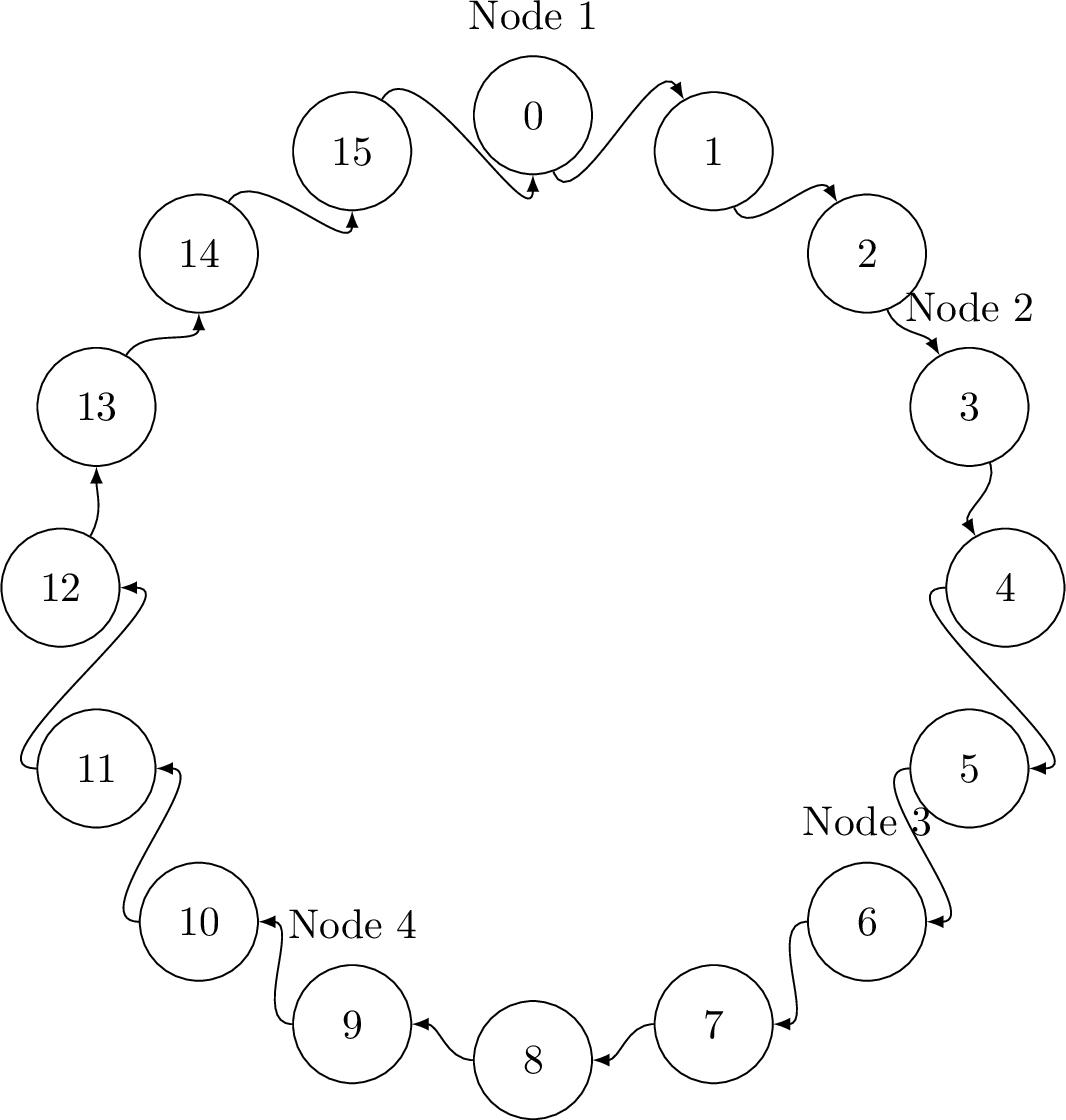
\includegraphics[width=0.45\textwidth]{fig/tex-grapics/chord.pdf.png}
    \caption{Chord Setup}
    \label{fig:chord}
  \end{figure}
\end{frame}

\begin{frame}
  \frametitle{P2P Chord}
  \framesubtitle{Fingertable}
  \begin{itemize}
    \item $log(n)$ Einträge
    \item $(n + 2^{(i-1)}) \mod 2^m$
    \item Lässt schnelle Suche zu (im Vergleich zur linearen)
  \end{itemize}
\end{frame}

\begin{frame}
  \frametitle{P2P Chord}
  \framesubtitle{Cassandra}
  \begin{itemize}
    \item NoSQL-Datenbanksystem
    \item Partitionierungsstrategie
    \begin{itemize}
      \item Range-based Sharding
      \item Hash-based Sharding
    \end{itemize}
    \item Replikationsstrategie
    \item Datenmodell
    \item Gossip-Protokoll (statt Fingertable für Routing-Aufbau)
    \item Hinted Handoff
    \item Repair und Anti-Entropy
  \end{itemize}
\end{frame}

% ------------------------------------------------------------------------------
% Fin
\end{document}